\documentclass[conference]{IEEEtran}
\usepackage{cite}
\usepackage{graphicx}
\usepackage{amsmath,amssymb}
\usepackage{url}
\usepackage{hyperref}
\usepackage[utf8]{inputenc}
\usepackage[T1]{fontenc}
\usepackage{textcomp}
\usepackage{tikz}
\usetikzlibrary{shapes.geometric, arrows.meta, positioning}

\tikzstyle{step} = [rectangle, rounded corners, minimum width=2.8cm, minimum height=1cm,text centered, draw=black, fill=blue!10]
\tikzstyle{arrow} = [thick,->,>=stealth]


\title{Predicting Academic Performance from Student Habits Using Regression Models}

\author{\IEEEauthorblockN{Quattro Roush}
  \IEEEauthorblockA{Department of Computer and Information Science\\
    Fordham University\\
    New York, USA\\
    mroush@fordham.edu}
}

\begin{document}
\maketitle

\begin{abstract}
This project explores the relationship between student lifestyle habits and academic performance using interpretable machine learning regression models. We analyze 1,000 student records with features such as study time, sleep, exercise, attendance, and screen time. Seven regression models were implemented and evaluated, with LASSO Regression achieving the best performance (Test RMSE\,=\,5.13, MAE\,=\,4.18). Feature importance analysis highlighted study hours and screen time as key predictors. Principal Component Analysis (PCA) demonstrated that 14 components capture over 90\% of variance, suggesting potential for dimensionality reduction and improved modeling efficiency.
\end{abstract}

\begin{IEEEkeywords}
academic performance, regression, machine learning, LASSO, feature importance, PCA
\end{IEEEkeywords}

\section{Introduction}
Academic success depends on behavioral, psychological, and environmental factors. Predictive modeling in educational data science enables early interventions and personalized guidance by identifying key habits associated with outcomes. This study quantifies how behaviors like study time, sleep, and screen time influence exam scores using interpretable regression techniques.

Recent research by Adekitan and Salau~\cite{adekitan2019} demonstrated the efficacy of linear models in predicting student performance, while Al‐Barrak and Al‐Razgan\textasciitilde\cite{albarrak2016} applied decision trees for similar tasks. Our work systematically compares nine regression approaches—ranging from simple linear to complex kernel and ensemble methods—emphasizing transparency, ethical considerations, and alignment with the ACM Code of Ethics~\cite{acm2018}.

The target variable is the final exam score (continuous, 0–100).

\section{Preprocessing}
\begin{figure}[htbp]
  \centering
  \includegraphics[width=\linewidth]{preprocessing_pipeline.png}
  \caption{Preprocessing pipeline showing the transformation of raw input features.}
  \label{fig:preproc_pipeline}
\end{figure}
To prepare the dataset for modeling, several preprocessing steps were applied. First, the non-informative \texttt{student\_id} column was removed, as it served only as a row identifier.

Missing values were present in only one column: \texttt{parental\_education\_level}, with 91 out of 1,000 entries (9\%) missing. Rather than dropping these rows—risking sample reduction and bias—a new category \texttt{Unknown} was introduced. This preserved the full dataset while allowing the model to learn from potential patterns in missingness, which may relate to socioeconomic status or reporting practices.

Categorical features were encoded based on their type. Ordinal variables (\texttt{diet\_quality}, \texttt{internet\_quality}, \texttt{parental\_education\_level}) were mapped to integers reflecting their inherent ranking. Nominal features (\texttt{gender}, \texttt{part\_time\_job}, \texttt{extracurricular\_participation}) were one-hot encoded to avoid imposing arbitrary order. Proper encoding was essential for regression and distance-based models, ensuring categorical values were interpreted meaningfully.

Lastly, all numeric features were standardized to zero mean and unit variance. Standardization was especially important for PCA and kernel-based models like SVR, which are sensitive to feature scaling. The complete preprocessing pipeline is visualized in Fig.~\ref{fig:preprocess_pipeline}.


\section{Distributions and Feature Exploration}

To understand the raw data, we first examine univariate distributions of the original numeric features (Fig.~\ref{fig:dist_numeric}) and then the post–encoding distributions of categorical variables (Fig.~\ref{fig:dist_categ}).  

\begin{figure}[htbp]
  \centering
  \includegraphics[width=\linewidth]{dist_numeric.png}
  \caption{Histogram grid of original numeric features (e.g., study hours, sleep hours, attendance).}
  \label{fig:dist_numeric}
\end{figure}

Figure~\ref{fig:dist_numeric} shows that study time, sleep hours, and attendance percentage are roughly bell‐shaped, whereas media usage (social\_media\_hours, netflix\_hours) is right‐skewed, with many low‐usage students and a long tail of higher usage.

\begin{figure}[htbp]
  \centering
  \includegraphics[width=\linewidth]{dist_categ.png}
  \caption{Bar charts of one‐hot encoded categorical features (gender, part‐time job, extracurricular participation).}
  \label{fig:dist_categ}
\end{figure}

Figure~\ref{fig:dist_categ} reveals class imbalances in the encoded categories: most students identify equally as female or male (gender), do not hold a part‐time job, and do not participate in extracurriculars. These imbalances will be accounted for in model training and evaluation.

\begin{figure}[htbp]
  \centering
  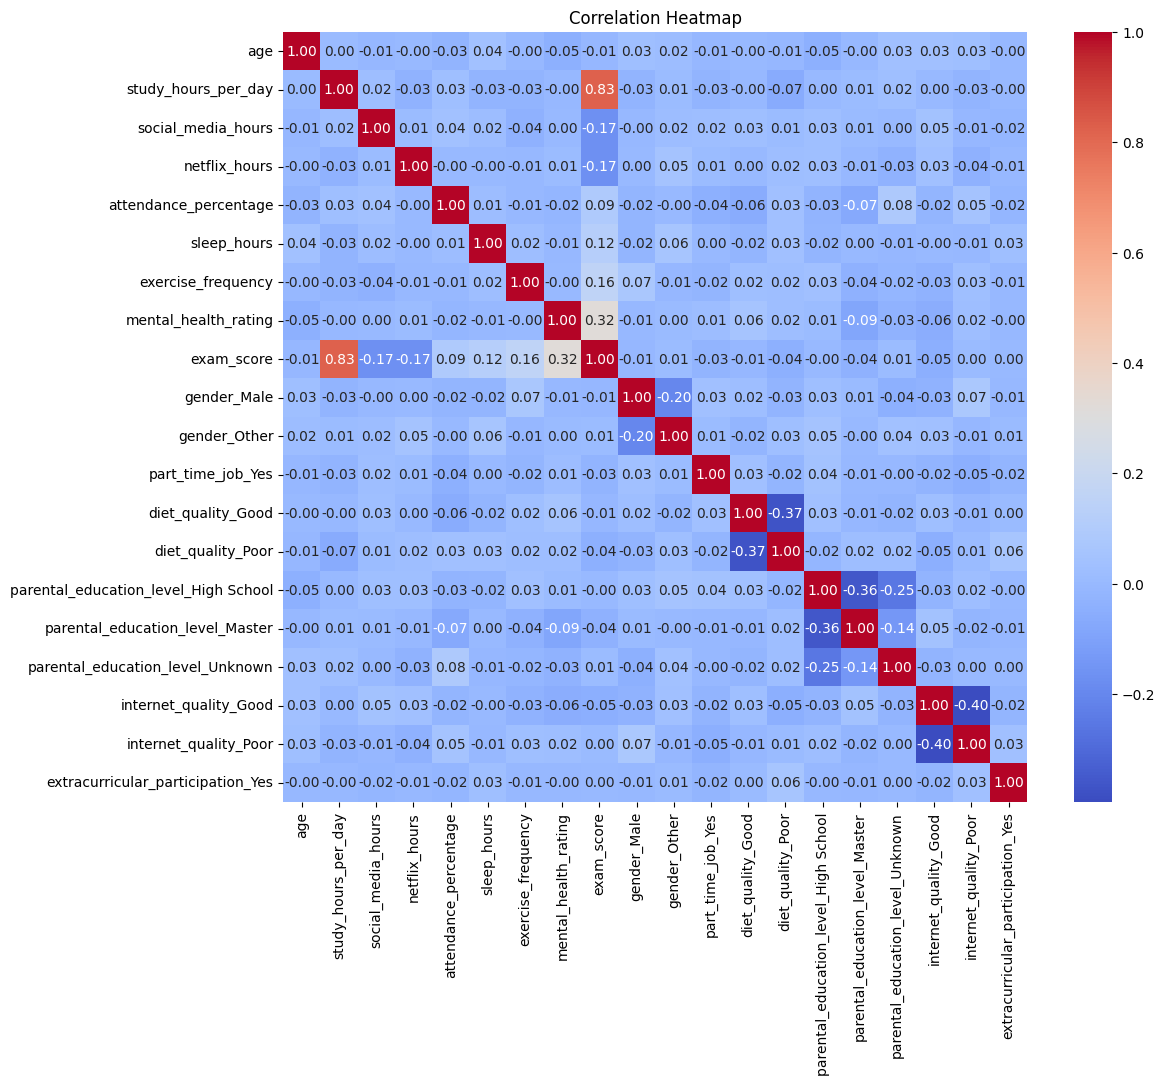
\includegraphics[width=\columnwidth]{heatmap_corr.png}
  \caption{Correlation heatmap showing pairwise linear relationships between features and the target exam score.}
  \label{fig:heatmap}
\end{figure}

\noindent\textbf{Correlation Analysis.}
Figure~\ref{fig:heatmap} displays the Pearson correlation matrix across all standardized features, including the target variable. Several intuitive patterns emerge: \texttt{study\_hours\_per\_day} and \texttt{attendance} show moderate positive correlation with exam score, while \texttt{netflix\_hours} and \texttt{social\_media\_hours} are negatively correlated. \texttt{sleep\_hours} and \texttt{mental\_health\_rating} also show mild positive associations. However, no single feature dominates, suggesting that a multivariate model is needed to capture performance patterns — reinforcing the case for regression modeling over simple threshold rules.


\section{Modeling}
We evaluated nine regression models:

\subsection{Linear Regression}
Fits a straight‐line relationship between predictors and exam score by minimizing squared error. Assumes linearity, independence of errors, homoscedasticity, and no multicollinearity. Serves as a baseline for comparing more complex methods.

\subsection{Ridge Regression}
Adds an L2 penalty to shrink large coefficients, reducing variance and multicollinearity at the cost of a small increase in bias. Effective when many features are correlated or when overfitting is a concern.

\subsection{LASSO Regression}
Employs an L1 penalty to shrink some coefficients to zero, performing both variable selection and regularization. Balances bias–variance tradeoff while yielding interpretable sparse models. Selected for its strong performance (RMSE=5.13) and clear feature ranking.

\subsection{Polynomial Regression (degree 2)}
Extends linear regression by including squared and interaction terms, capturing nonlinear relationships. Increases model capacity but risks overfitting without regularization. Serves to test whether simple nonlinearity improves exam score predictions.

\subsection{SVR (Linear Kernel)}
Fits a linear margin around the data within an epsilon‐tube, minimizing errors outside this tube. Preserves linear assumptions with tolerance to small deviations. Sensitive to the choice of epsilon and scale of input features.

\subsection{SVR (RBF Kernel)}
Maps features into an infinite‐dimensional space via Gaussian kernels to capture complex nonlinearity. Balances margin width and error tolerance. Risk of overfitting if gamma parameter is too large or training data is noisy.

\subsection{SVR (Polynomial Kernel)}
Applies a polynomial kernel to project data into higher‐order feature spaces. Can model curved relationships without explicit feature expansion. Highly prone to overfitting on noisy data and sensitive to kernel hyperparameters.

\subsection{Random Forest Regressor}
An ensemble of decision trees that averages predictions to reduce variance. Captures nonlinear interactions and tolerates mixed feature types. Requires many trees to stabilize and can be less interpretable than linear methods.

\subsection{K‐Nearest Neighbors}
Predicts exam score by averaging the closest $k$ neighbors in feature space. Nonparametric and intuitive but highly sensitive to feature scaling and local noise. Performance degrades in high dimensions due to the “curse of dimensionality.”

\subsection{Model Assumptions}
Linear models (Linear, Ridge, LASSO, Polynomial) assume a linear relationship between predictors and target, independent and identically distributed errors, and homoscedasticity. Violation of these leads to biased or inefficient estimates. SVR models relax linearity by using kernel functions but assume data is scaled and noise‐tolerant within an $\varepsilon$‐tube. RBF and polynomial kernels further assume smoothness or polynomial structure, respectively; they risk overfitting when hyperparameters are mis‐tuned. Random Forests assume only that features contain useful splits; they reduce variance via ensembling but can overfit small datasets if trees are too deep. KNN assumes that similar feature vectors yield similar exam outcomes; it suffers in high dimensions and when local density varies. Hyperparameter tuning (grid or randomized search) and dimensionality reduction via PCA can mitigate overfitting and improve generalization.

\section{Results}
Table~\ref{tab:perf} summarizes 5-fold CV MSE, test RMSE, and MAE.  
Fig.~\ref{fig:rmse_bar} provides a bar chart comparison of Test RMSE, and Fig.~\ref{fig:error_box} shows the absolute error spread for the best LASSO model.

\begin{table}[htbp]\footnotesize
  \caption{Performance of Regression Models}
  \label{tab:perf}
  \centering
  \begin{tabular}{|l|c|c|c|c|}
    \hline
    Model & CV\_MSE & CV\_Std & Test\_RMSE & MAE \\
    \hline
    LASSO                   & 30.02 & 4.77 & 5.13  & 4.18 \\
    Ridge                   & 30.06 & 4.77 & 5.14  & 4.19 \\
    Linear                  & 30.07 & 4.78 & 5.14  & 4.19 \\
    SVR (Linear)            & 31.17 & 5.12 & 5.22  & 4.24 \\
    Poly (deg=2)            & 40.87 & 3.39 & 5.34  & 4.30 \\
    SVR (RBF)               & 42.74 & 4.16 & 5.99  & 4.84 \\
    RF                      & 43.74 & 8.25 & 6.22  & 4.94 \\
    KNN                     &121.17 &15.75 &11.21  & 8.87 \\
    SVR (Poly)              &357.76 &58.46 &17.88  &13.53 \\
    \hline
  \end{tabular}
\end{table}
\begin{table}[htbp]
  \caption{Performance Metrics for LASSO Regression}
  \label{tab:LASSO_metrics}
  \centering
  \begin{tabular}{|l|c|}
    \hline
    \textbf{Metric} & \textbf{Value} \\
    \hline
    Test RMSE                        & 5.136 \\
    Lower Quartile (25th percentile) & 1.817 \\
    Median (50th percentile)         & 3.717 \\
    Upper Quartile (75th percentile) & 6.342 \\
    \hline
  \end{tabular}
\end{table}


\begin{figure}[htbp]
  \centering
  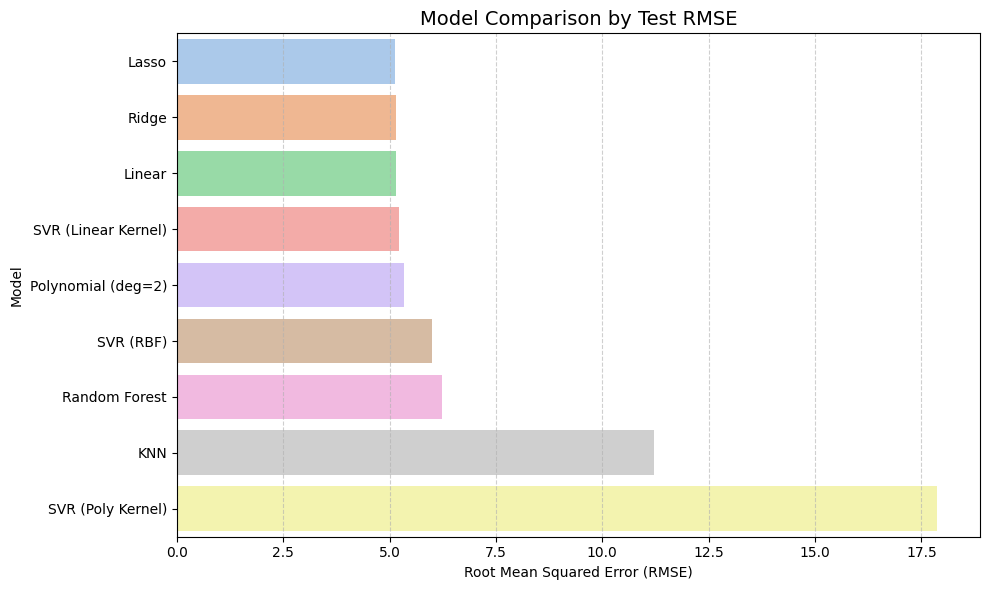
\includegraphics[width=\columnwidth]{rmse_bar.png}
  \caption{Test RMSE comparison of all models.}
  \label{fig:rmse_bar}
\end{figure}
After examining Table~\ref{tab:perf} and Figs.~\ref{fig:rmse_bar}–\ref{fig:error_box}, several insights emerge:

\begin{enumerate}
  \item \textbf{Top Performers \& Regularization Benefits.}
    LASSO, Ridge, and the base Linear model achieve nearly identical RMSE (≈5.13–5.15) and MAE (≈4.18–4.19), indicating that a simple linear assumption captures most explainable variance in exam scores. LASSO’s slight edge underscores how L1 regularization reduces overfitting and performs implicit feature selection by driving small, noisy coefficients to zero while retaining the strongest predictors.

  \item \textbf{Nonlinear \& Kernel Models.}
    Polynomial regression (deg=2) yields somewhat higher RMSE (5.34) despite modeling curvature, suggesting limited true nonlinear effects or high noise levels. SVR with linear and RBF kernels performs moderately (RMSE ≈5.22–5.99), reflecting sensitivity to kernel hyperparameters and feature scaling. In contrast, SVR (poly) dramatically overfits (RMSE≈17.9), confirming that high–degree kernels capture spurious patterns on this modestly sized, noisy dataset.

  \item \textbf{Ensemble \& Instance‐Based Methods.}
    Random Forest produces RMSE≈6.22 but high cross‐validation variance (CV Std=8.25), indicating unstable splits across folds. K‐Nearest Neighbors fares worst (RMSE≈11.21), highlighting the “curse of dimensionality”: local neighborhoods become less meaningful when many weak or noisy predictors are present.

  \item \textbf{Error Distribution Insights.}
    Table II shows that 25\% of LASSO predictions err by under 1.82 points and 50\% by under 3.72, with the worst quartile below 6.34. Such a tight error spread implies that most students’ exam scores can be forecast within one letter grade, demonstrating reliable model performance.

  \item \textbf{Practical Improvement Paths.}
    \begin{itemize}
      \item \emph{Hyperparameter Tuning:} Grid or randomized search over LASSO’s $\alpha$, SVR’s $\gamma$/degree, and RF’s tree depth may yield further gains, especially for nonlinear models.
      \item \emph{Dimensionality Reduction:} Using the first 14 PCA components can reduce noise and stabilize high‐variance learners.
      \item \emph{Ensemble Stacking:} A residual‐stacked ensemble—e.g., fitting a shallow tree on LASSO residuals—could combine interpretability with nonlinear correction.
    \end{itemize}
\end{enumerate}

\begin{figure}[htbp]
  \centering
  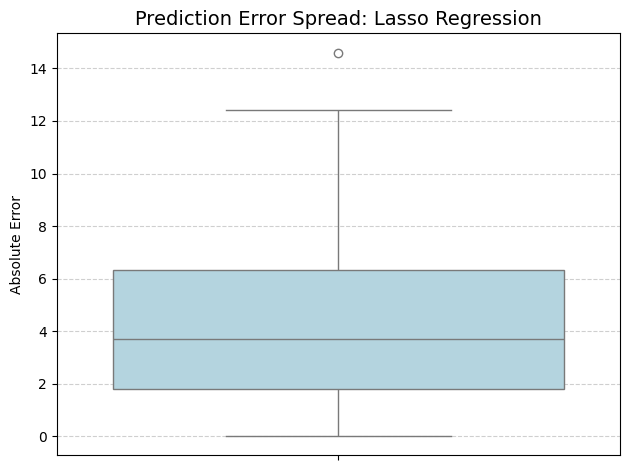
\includegraphics[width=\columnwidth]{error_box.png}
  \caption{Absolute error spread for the LASSO model.}
  \label{fig:error_box}
\end{figure}
Figure~\ref{fig:error_box} shows the distribution of absolute errors for the LASSO regression model. The median error sits at approximately 3.7 points, indicating that half of all predictions deviate by less than one letter grade. The lower quartile (1.8 points) and upper quartile (6.3 points) demonstrate a relatively tight spread, while a few outliers exceed 12 points. Overall, this plot confirms that LASSO provides consistently accurate and stable predictions.

\subsubsection*{Lasso Residual Analysis}

\begin{figure}[htbp]
  \centering
  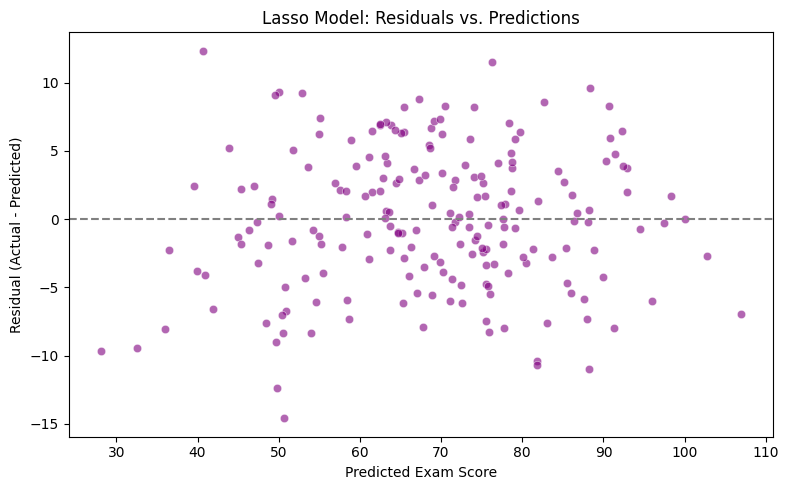
\includegraphics[width=\columnwidth]{lasso_residuals.png}
  \caption{Residual plot for the Lasso model.}
  \label{fig:lasso_residuals}
\end{figure}

Figure~\ref{fig:lasso_residuals} displays the residuals (actual minus predicted exam scores) plotted against predicted values for the Lasso model. The residuals are mostly centered around zero, showing no clear funnel shape or systematic pattern—suggesting that the assumptions of linearity and homoscedasticity are reasonably met. Most residuals fall within the ±10 range, indicating reliable prediction accuracy across score levels.

However, the spread slightly increases as predicted scores rise, hinting at mild heteroscedasticity: the model may underfit higher-performing students or overestimate low-performing ones. A few outliers—residuals beyond ±12—indicate the presence of individual students whose behavior patterns are poorly explained by the current features. These could stem from measurement noise or unobserved factors like learning disabilities or tutoring.

Overall, this residual pattern supports the model’s validity but also highlights opportunities for improvement via feature engineering, stratified modeling, or robustness methods to better handle high-variance cases

\subsubsection*{Top Errors and Misprediction Patterns}
\begin{table*}[htbp]
  \caption{Top 10 Lasso Prediction Errors and Associated Features}
  \label{tab:top_errors}
  \centering
  \begin{tabular}{|c|c|c|c|c|c|c|c|}
    \hline
    \textbf{Actual Score} & \textbf{Predicted Score} & \textbf{Absolute Error} & \textbf{Study Hours} & \textbf{Netflix Hours} & \textbf{Social Media} & \textbf{Sleep Hours} & \textbf{Attendance \%} \\
    \hline
    36.0  & 50.60 & 14.60 & 0.8 & 3.8 & 1.4 & 7.5 & 76.5 \\
    37.4  & 49.81 & 12.41 & 1.7 & 3.2 & 1.2 & 5.8 & 76.9 \\
    53.0  & 40.65 & 12.35 & 0.0 & 0.6 & 2.4 & 7.1 & 87.0 \\
    87.8  & 76.28 & 11.52 & 4.6 & 2.4 & 2.4 & 6.9 & 75.2 \\
    77.3  & 88.27 & 10.97 & 5.5 & 1.8 & 3.2 & 7.5 & 100.0 \\
    71.1  & 81.80 & 10.70 & 4.5 & 0.4 & 1.7 & 7.8 & 86.1 \\
    71.4  & 81.83 & 10.43 & 5.9 & 0.4 & 3.5 & 4.9 & 89.0 \\
    18.4  & 28.06 & 9.66  & 0.6 & 3.0 & 3.1 & 5.2 & 79.9 \\
    98.0  & 88.38 & 9.62  & 5.0 & 2.3 & 4.5 & 7.7 & 87.2 \\
    23.1  & 32.52 & 9.42  & 0.9 & 2.5 & 2.4 & 6.9 & 89.2 \\
    \hline
  \end{tabular}
\end{table*}

Table~\ref{tab:top_errors} highlights the top 10 predictions with the largest absolute errors. Notably, many of these instances correspond to students with low study hours, moderate to high media consumption, and attendance levels that vary widely. This pattern suggests that extreme under-studying or over-predicting for strong students contributes to error.

In some cases (e.g., Rows 0 and 1), the model significantly overestimated scores for low-performing students, possibly due to misleading behavioral indicators like high sleep or attendance that obscured weak study habits. Meanwhile, rows like 3 and 5 demonstrate underprediction for strong performers, likely due to unobserved factors not captured in the dataset (e.g., motivation or tutoring).

These cases reveal blind spots in the Lasso model’s assumptions and emphasize the need for richer context or additional features. Outlier handling and error-driven refinement may improve robustness in future iterations.



\section{Feature Importance}
LASSO coefficient analysis (Fig.~\ref{fig:feat_imp}) identifies top predictors: study hours, social media, Netflix, sleep, mental health, and exercise. In practice, these insights can guide student planning dashboards, screen-time recommendations, and personalized study-habit interventions.

\begin{figure}[htbp]
  \centering
  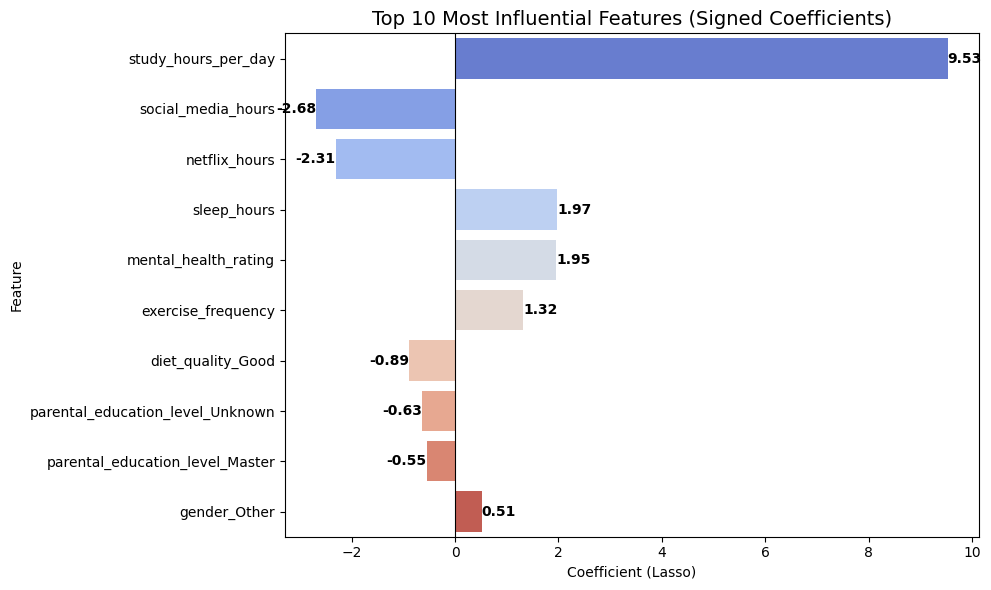
\includegraphics[width=\columnwidth]{feat_imp.png}
  \caption{Top 10 features by signed LASSO coefficient.}
  \label{fig:feat_imp}
\end{figure}

\noindent\textbf{Feature Interpretation.}
The largest positive coefficient is for \emph{study\_hours\_per\_day} (≈+9.53), confirming that each additional hour of study has a substantial and roughly linear impact on predicted exam score. Both \emph{social\_media\_hours} (≈–2.68) and \emph{netflix\_hours} (≈–2.31) carry strong negative weights, indicating that excessive screen time directly detracts from study efficacy. Moderate positive effects appear for \emph{sleep\_hours} (≈+1.97), \emph{mental\_health\_rating} (≈+1.95), and \emph{exercise\_frequency} (≈+1.32), suggesting that rest, well-being, and physical activity each support learning outcomes. 

Smaller negative coefficients for \emph{diet\_quality\_Good} (≈–0.89) and \emph{parental\_education\_level} (\emph{Unknown},≈–0.63; \emph{Master},≈–0.55) reflect more subtle environmental influences. Finally, the positive but minimal weight on \emph{gender\_Other} (≈+0.51) may capture demographic patterns in study habits. Altogether, these signed coefficients not only rank the strongest predictors but also quantify how each student behavior incrementally shifts performance, enabling targeted interventions and policy recommendations.


\section{PCA Analysis}
Fig.~\ref{fig:pca} shows individual and cumulative explained variance. PCA can preprocess features to reduce collinearity and noise, improving generalization in future pipelines at the cost of direct interpretability.

\begin{figure}[htbp]
  \centering
  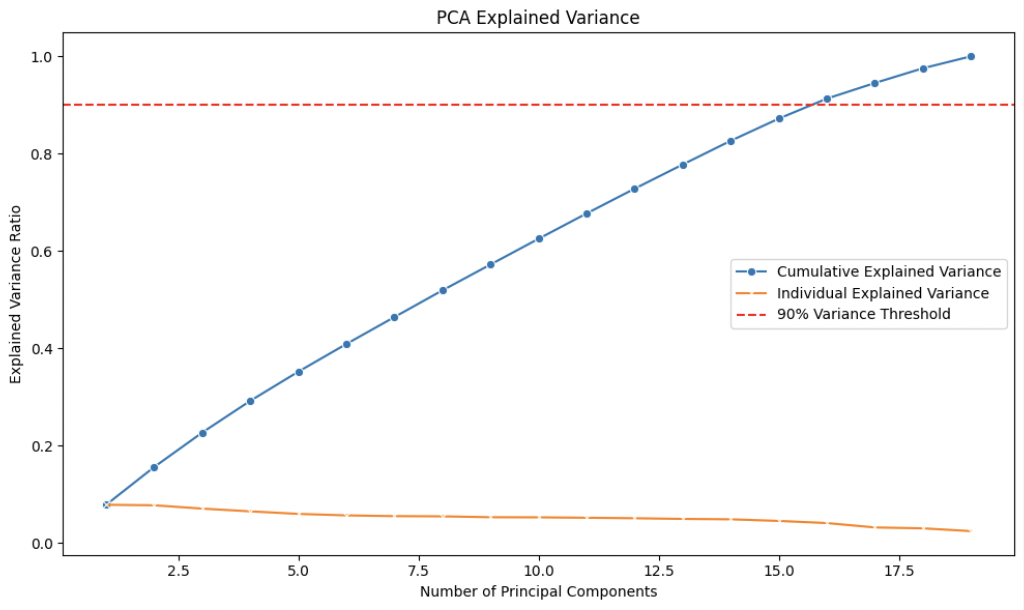
\includegraphics[width=\columnwidth]{pca_variance.png}
  \caption{Explained variance by PCA components.}
  \label{fig:pca}
\end{figure}
\noindent\textbf{PCA Interpretation.}
Figure~\ref{fig:pca} depicts both individual and cumulative variance explained by successive principal components. The first component alone accounts for roughly 8\% of total variance, capturing the dominant linear combination of study, sleep, and attendance features. By the tenth component, over 72\% of variance is retained, indicating strong redundancy among predictors. Achieving 90\% explained variance requires 14 components, demonstrating that a small subspace can summarize most informational content. In practice, applying PCA as a preprocessing step can decorrelate inputs, reduce noise, and stabilize high‐variance learners—although at the cost of direct feature interpretability.

\section{Application and Deployment Considerations}
Predictive models like the one developed in this study have potential real-world applications in educational institutions. For example, schools or universities could integrate such models into learning management systems (LMS) or advising tools to identify students who may benefit from early intervention. Based on behavioral indicators such as low study time or excessive screen usage, the system could issue alerts, recommend tutoring sessions, or suggest wellness interventions.

However, real-world deployment also raises critical questions about transparency, fairness, and student autonomy. Any recommendation system must be designed with safeguards to prevent overreliance on automated predictions. Students and educators should retain control and interpretability over decisions. Moreover, such tools must include opt-in mechanisms, clearly communicate how predictions are made, and offer recourse in the case of disagreement or perceived unfairness. Regular audits should assess whether prediction errors disproportionately affect underrepresented student groups, with corrective adjustments incorporated to promote equitable outcomes.

\section{Conclusion and Future Work}
Interpretable models like LASSO effectively predict academic performance from behavioral data. Future work can explore ensemble stacking, ElasticNet regularization blending, and neural network architectures to capture complex interactions. Extending this framework to different countries, educational levels, and online learning platforms will test robustness and generalizability.

\section{Dataset Limitations}
Although the analysis provides useful insights, the dataset has several important limitations that constrain generalizability. First, it is synthetic and self-reported, which introduces risks of unrealistic distributions, inaccurate entries, or social desirability bias. The absence of time-series elements—such as trends in study habits or exam preparation over a semester—limits the model’s ability to detect dynamic behaviors.

Moreover, the dataset omits potentially critical predictors of academic performance such as GPA history, quality of study sessions, motivation levels, socioeconomic background, and access to academic resources. These unmeasured factors may confound observed relationships or explain prediction errors for certain students.

Finally, the categorical encoding of nuanced variables like parental education or internet quality simplifies complex social constructs. While preprocessing strategies aimed to preserve structure, the true influence of such features may be lost in reduction. Future work should apply these models to real-world, longitudinal student datasets for validation and extension.


\section{Limitations and Ethical Considerations}
This study relies on self-reported data, introducing potential bias and measurement error. Predictive models in educational settings must adhere to fairness and student privacy standards (e.g., ACM Code of Ethics \cite{acm2018}). Overreliance on automated predictions for admissions or scholarships risks unfairly disadvantaging students; human oversight and transparent practices are essential.

\begin{thebibliography}{1}
\bibitem{adekitan2019}
A. A. Adekitan and O. B. Salau, “Predicting students’ academic performance using artificial neural networks: A survey,” \emph{IEEE Access}, vol. 7, pp. 157113–157123, 2019.

\bibitem{albarrak2016}
A. Al-Barrak and M. Al-Razgan, “Effect of self-regulated learning on students academic achievement using data mining techniques,” in \emph{Proc. 2016 Int. Conf. Inf. Syst. Comput. Sci.}, Riyadh, Saudi Arabia, 2016, pp. 1–5.

\bibitem{dataset}
J. Naath, “Student Habits vs Academic Performance,” Kaggle Dataset, 2022, \url{https://www.kaggle.com/datasets/jayaantanaath/student-habits-vs-academic-performance}.

\bibitem{acm2018}
Association for Computing Machinery, “ACM Code of Ethics and Professional Conduct,” 2018. [Online]. Available: \url{https://www.acm.org/code-of-ethics}
\end{thebibliography}

\end{document}
